\documentclass{../../../../style/mkimain}

\series{4}
\month{květen}
\year{2023}

\begin{document}
%<*header>
\section*{IV.U1 Header4-U1}
%</header>
%<*task>

\noindent K následujícím obrázkům přiřaďte jev, nebo objekt, který zachycuje.

\vspace{0.5cm}
\begin{mdframed}[frametitle={Díla}, frametitlealignment=\center, innerbottommargin=5px]
    \begin{center}
        speciální~princip~relativity, gravitační~zákon, elektromagnetická~indukce, stanovení~teploty~černé~díry, myšlenkový~experiment~s~kočkou~v~krabici, teorie~radioaktivity
    \end{center}
\end{mdframed}
\vspace{1cm}
\begin{figure}[H]
  \minipage{0.3\textwidth}
    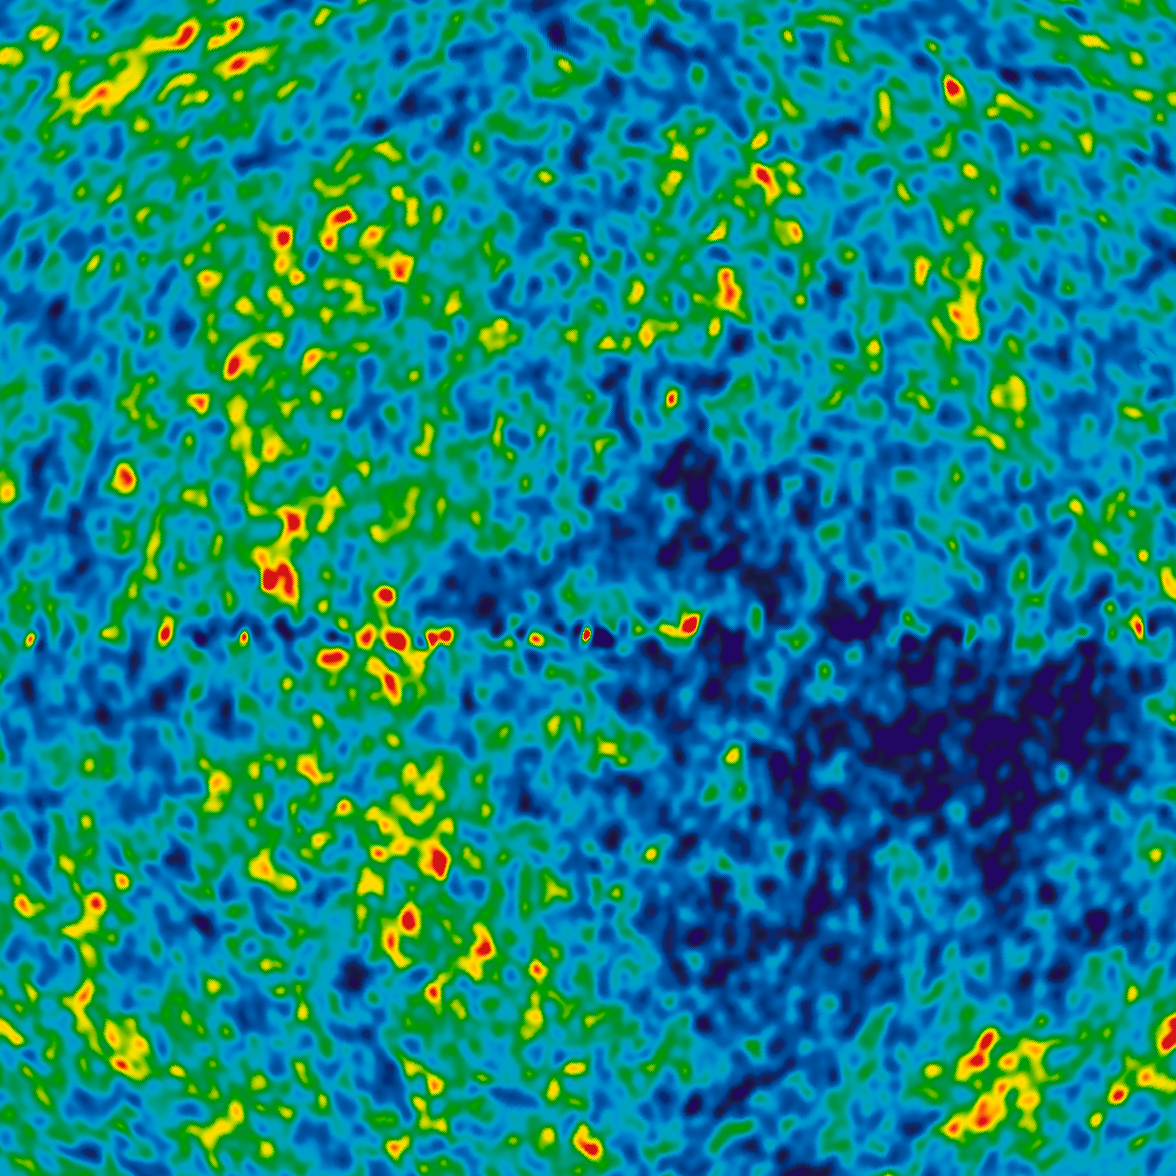
\includegraphics[width=\linewidth]{images/reliktni-zareni.png}
    \begin{center}
      1\footnotemark[1]
      \end{center}
  \endminipage\hfill
  \minipage{0.3\textwidth}
    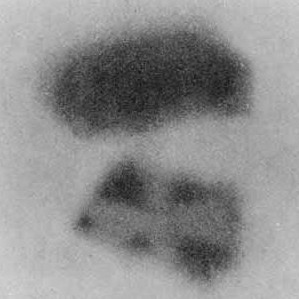
\includegraphics[width=\linewidth]{images/becquerel.jpg}
    \begin{center}
      2\footnotemark[2]
      \end{center}
  \endminipage\hfill
  \minipage{0.3\textwidth}%
    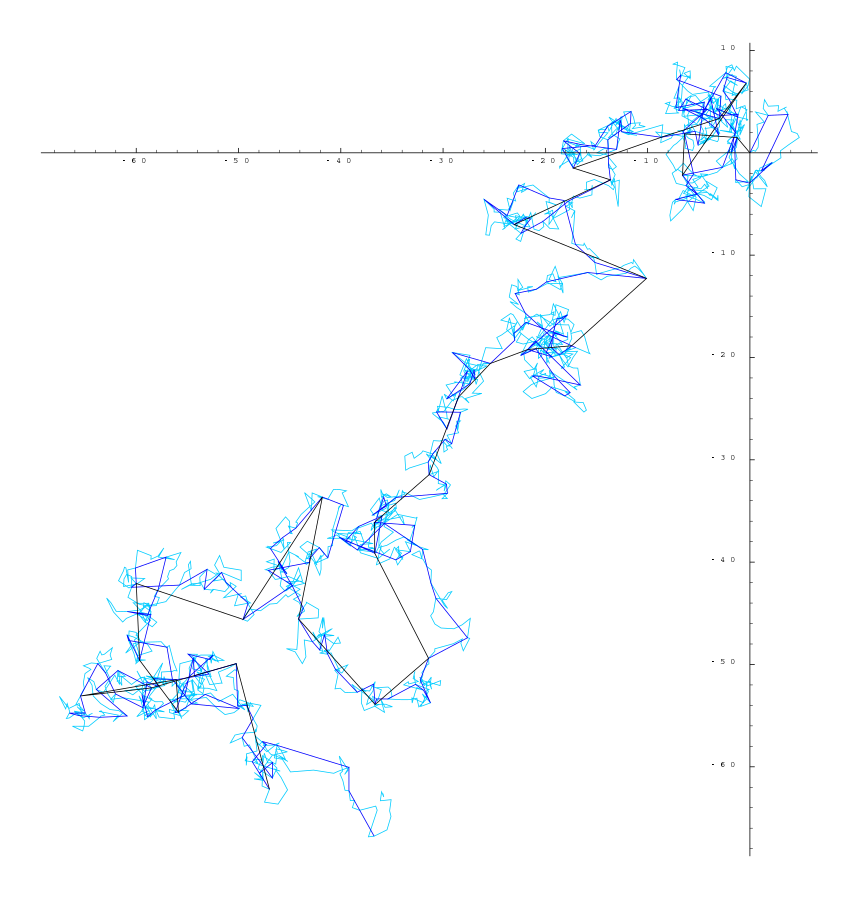
\includegraphics[width=\linewidth]{images/brownuv-pohyb.png}
    \begin{center}
    3\footnotemark[3]
    \end{center}
  \endminipage
\end{figure}
\vspace{0.5cm}
\begin{figure}[H]
  \minipage{0.3\textwidth}
    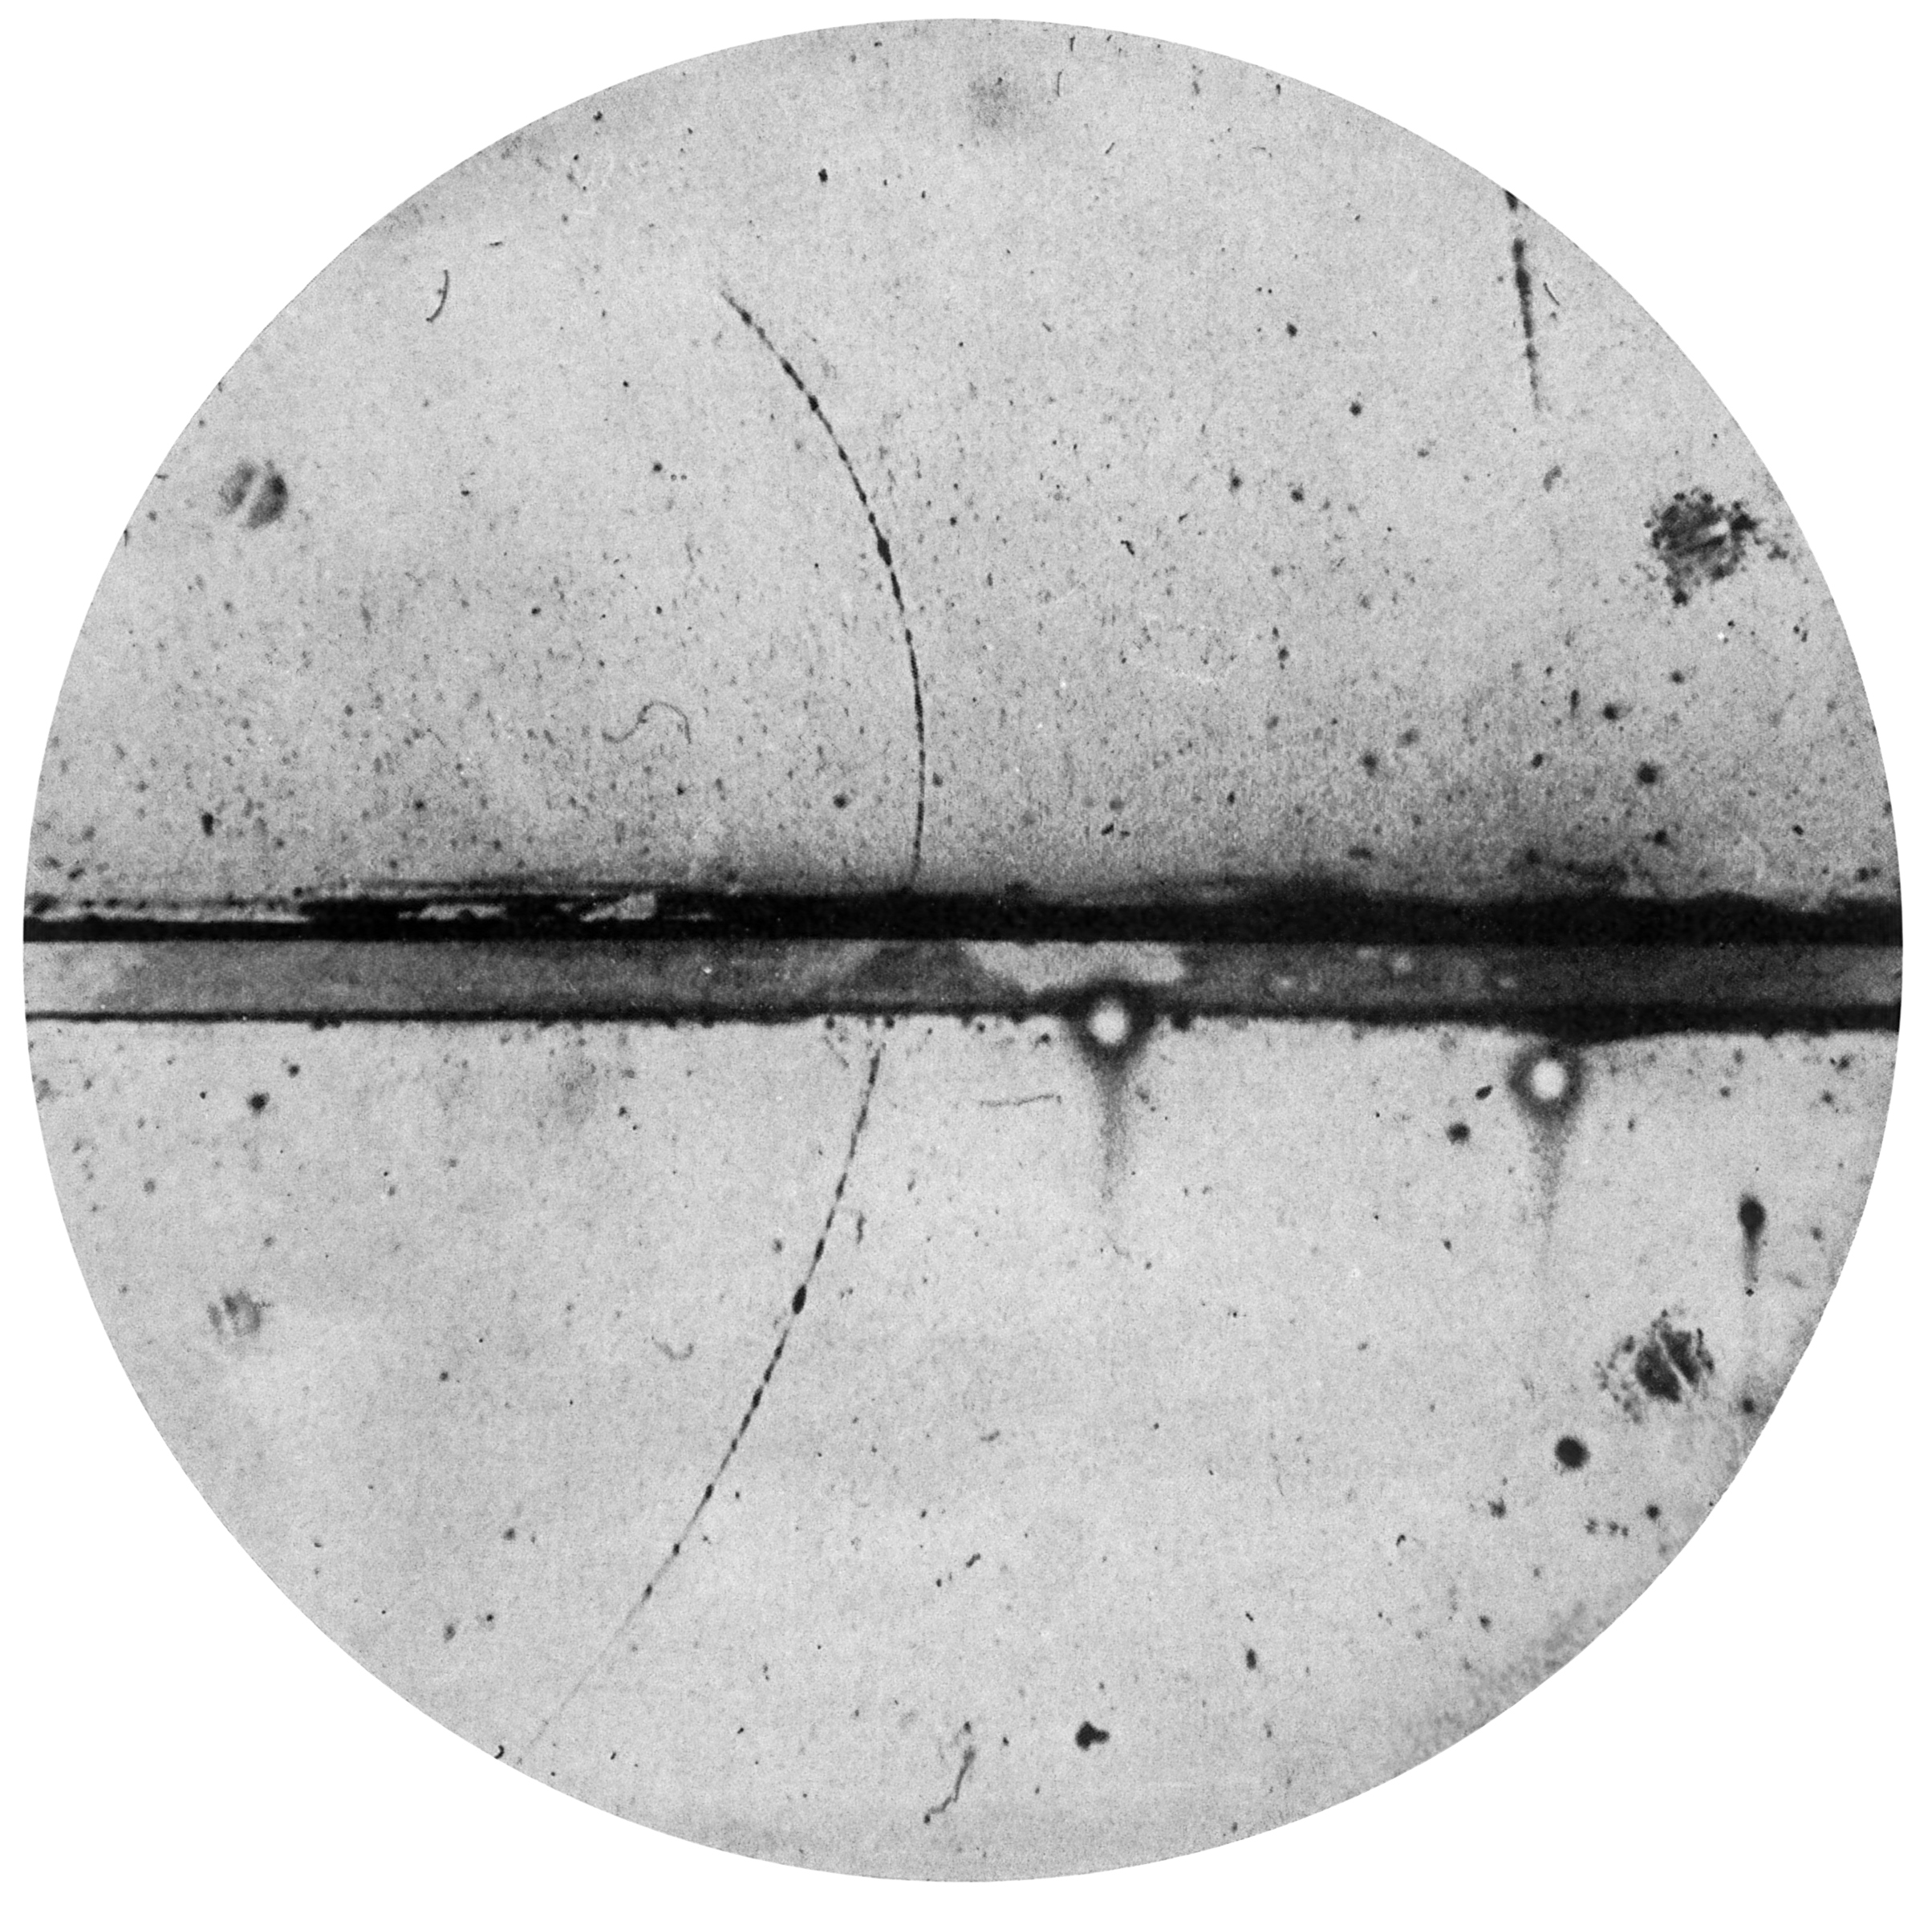
\includegraphics[width=\linewidth]{images/pozitron.jpg}
    \begin{center}
      4\footnotemark[4]
      \end{center}
  \endminipage\hfill
  \minipage{0.3\textwidth}
    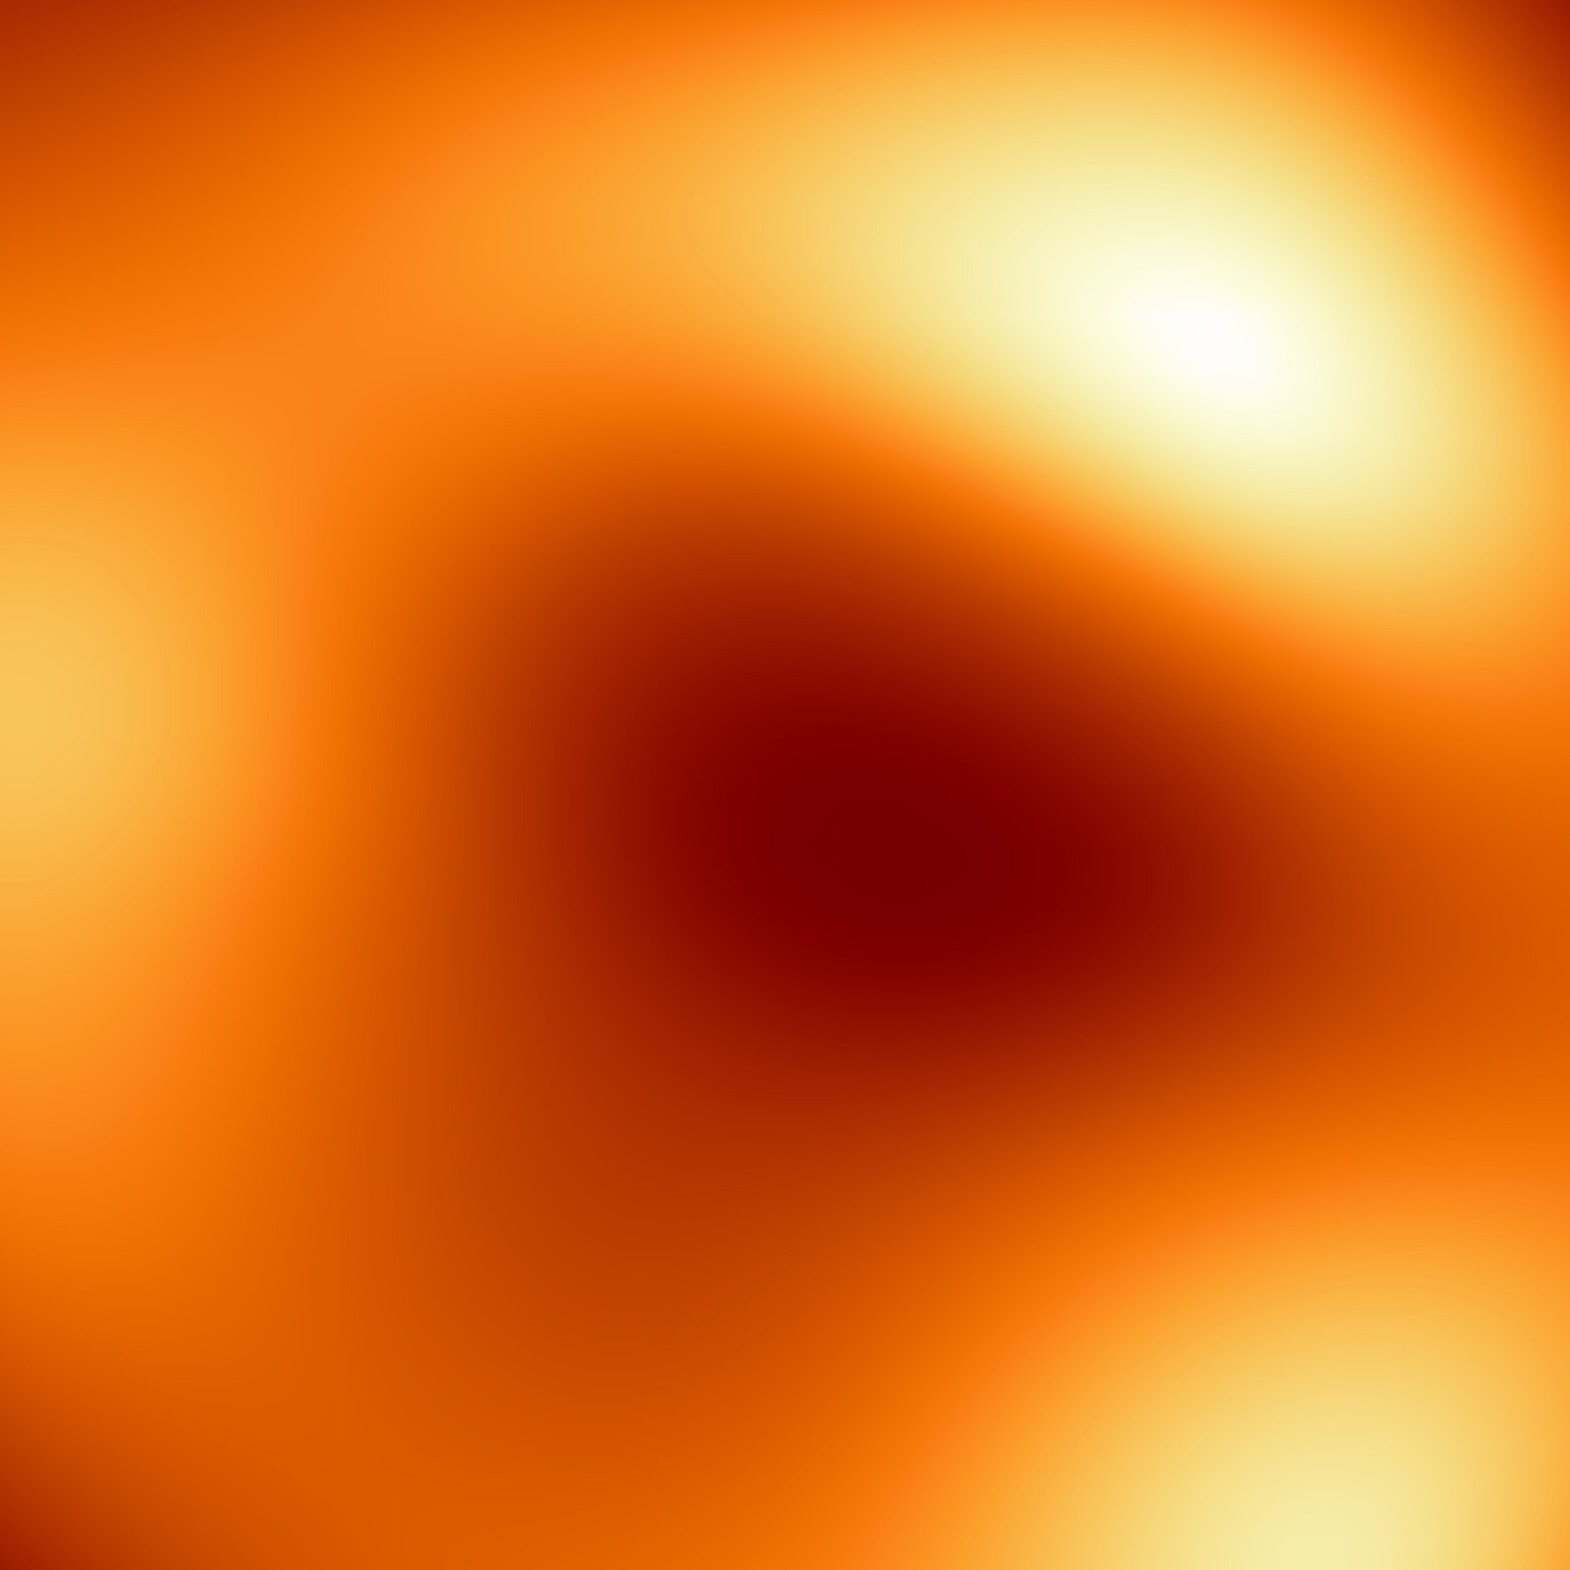
\includegraphics[width=\linewidth]{images/sagittarius.jpg}
    \begin{center}
      5\footnotemark[5]
      \end{center}
  \endminipage\hfill
  \minipage{0.3\textwidth}%
    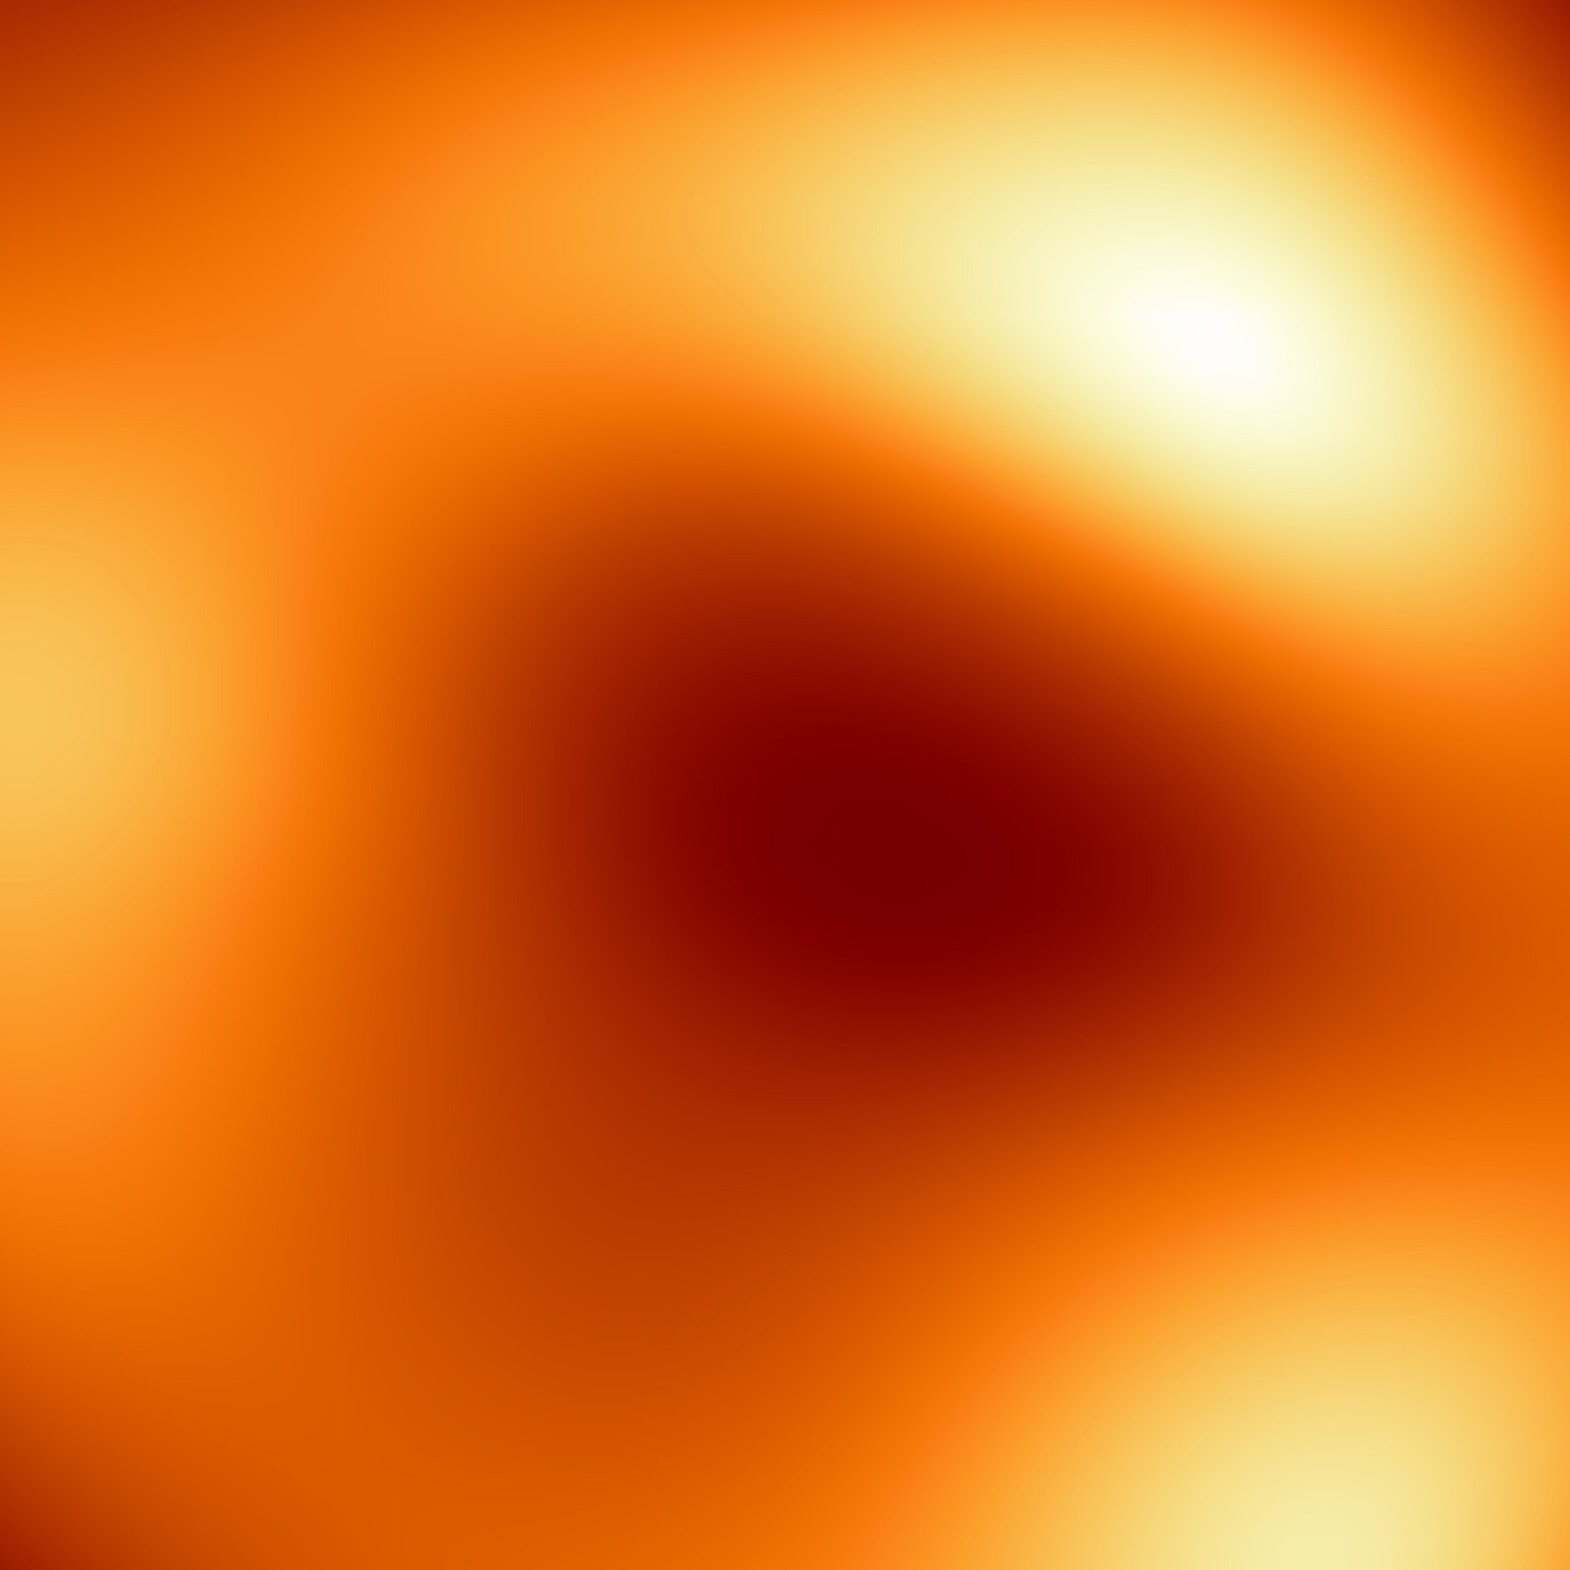
\includegraphics[width=\linewidth]{images/sagittarius.jpg}
    \begin{center}
      6\footnotemark[6]
      \end{center}
  \endminipage
\end{figure}

\footnotetext[1]{Credit: NASA/WMAP Science Team}
\footnotetext[2]{}
\footnotetext[3]{}
\footnotetext[4]{Credit: EHT Collaboration}
\footnotetext[5]{}
\footnotetext[6]{}

%</task>
\end{document}
